%----------------------------------------------------------------------------------------
%	PACKAGES AND OTHER DOCUMENT CONFIGURATIONS
%----------------------------------------------------------------------------------------

\documentclass[letter,11pt]{scrartcl}

% Fonts, Line-Spacing, and Indentation
\usepackage{fourier}
\usepackage[T1]{fontenc}
\usepackage{microtype}
\usepackage{color}
\setlength\parindent{0pt}
\usepackage{booktabs}
\usepackage{hyperref}
\usepackage{titlesec}
\usepackage[hang,small,labelfont=bf,up,textfont=it,up]{caption}
\usepackage{subfig}
\usepackage{array}
\usepackage[table]{xcolor}

%------------------------------------------------------

% Symbols
\usepackage{amssymb,amsmath,amsthm}
\usepackage{MnSymbol}
\usepackage{lambda}
\renewcommand{\progfontsize}{\normalsize}
\providecommand{\abs}[1]{\lvert#1\rvert}
\providecommand{\norm}[1]{\lVert#1\rVert}

%------------------------------------------------------

% Sections and Margins
\usepackage{chngcntr}
\usepackage{scrextend}
\usepackage{multicol}
\setlength{\columnsep}{1cm}

%------------------------------------------------------

% Venn Diagrams and Images
\usepackage{tikz}
\usetikzlibrary{arrows,backgrounds,petri,shapes,topaths}
\usepackage{float}
\usepackage{wrapfig}
\usepackage{makecell}

%------------------------------------------------------

% Margins
\usepackage[hmarginratio=1:1,top=10mm,columnsep=20pt]{geometry}

%------------------------------------------------------

% Custom Theorem Setup
\newtheorem{innercustomthm}{Theorem}
\newenvironment{customthm}[1]
  {\renewcommand\theinnercustomthm{#1}\innercustomthm}
  {\endinnercustomthm}


%------------------------------------------------------

% Custom macros
\definecolor{headFont}{RGB}{255,255,255}
\definecolor{headBack}{RGB}{100,100,100}

\newcommand{\inlinecode}{\texttt}
\newcommand{\zwei}[2]{\rowcolor{headBack}\textbf{\textcolor{headFont}{#1}} &
  \textbf{\textcolor{headFont}{#2}} \\}
\newcommand{\drei}[3]{\rowcolor{headBack}\textbf{\textcolor{headFont}{#1}} &
  \textbf{\textcolor{headFont}{#2}} & \textbf{\textcolor{headFont}{#3}} \\}
\newcommand{\vier}[4]{\rowcolor{headBack}\textbf{\textcolor{headFont}{#1}} &
  \textbf{\textcolor{headFont}{#2}} & \textbf{\textcolor{headFont}{#3}} &
  \textbf{\textcolor{headFont}{#4}} \\ }
\newcommand{\neun}[9]{\rowcolor{headBack}\textbf{\textcolor{headFont}{#1}} &
  \textbf{\textcolor{headFont}{#2}} & \textbf{\textcolor{headFont}{#3}} &
  \textbf{\textcolor{headFont}{#4}} & \textbf{\textcolor{headFont}{#5}} &
  \textbf{\textcolor{headFont}{#6}} & \textbf{\textcolor{headFont}{#7}} &
  \textbf{\textcolor{headFont}{#8}} & \textbf{\textcolor{headFont}{#9}} \\}
\newcommand{\codeinfo}[4]{\hline{#1} & {#2} & {$#3$} & {$#4$} \\}
\newcommand{\edgeinfo}[2]{\hline{#1} & {$\lbrace #2\rbrace$} \\}
\newcommand{\wsinfo}[3]{\hline{#1} & {#2} & {#3} \\}


%----------------------------------------------------------------------------------------
%	TITLE SECTION
%----------------------------------------------------------------------------------------

\title{
  \normalfont \normalsize
  \textsc{Data Structures - CS 261 (Spring 2015)} \\
  \huge Assignment \#7 -- Solutions
}

\author{Keeley Abbott
\\ Theodore Duchow-Pressley}

\date{\normalsize\today}

%------------------------------------------------------

\begin{document}

\maketitle

%----------------------------------------------------------------------------------------
%	ARTICLE CONTENT
%----------------------------------------------------------------------------------------

\section[question_1]{In searching for a good hash function over the set of integer values,
  one student thought he could use the following: \\
\-\hspace{2cm}\prog{int index = (int) cos(value); // Cosine of 'value'} \\
What was wrong with this choice?}

The possible integers derived from \prog{(int)} \prog{math.cos(value)} are
$\lbrace -1, 0, 1 \rbrace$, which would result in a high rate of collision.

%------------------------------------------------------

\section[question_2]{Can you come up with a perfect hash function for the
  names of days of the week? The names of the months of the year? Assume a
  table size of 10 for days of the week and 15 for names of the months. In
  case you cannot find any perfect hash functions, we will accept solutions
  that produce a small number of collisions (< 3).}

There are many solutions for this problem, but for simplicity we began by
using the sum of the first three letters of each day of the week (since each
of these is unique to begin with):

\begin{table}[H]
  \centering
  \begin{tabular}{ | c | c | c | c | }
    \hline
    \vier{Day of the week}{First three}{Values of letters}{Sum of letters}
    \codeinfo{Monday}{MON}{12 + 14 + 13}{39}
    \codeinfo{Tuesday}{TUE}{19 + 20 + 4}{43}
    \codeinfo{Wednesday}{WED}{22 + 4 + 3}{29}
    \codeinfo{Thursday}{THU}{19 + 7 + 20}{46}
    \codeinfo{Friday}{FRI}{5 + 17 + 8}{30}
    \codeinfo{Saturday}{SAT}{18 + 0 + 19}{37}
    \codeinfo{Sunday}{SUN}{18 + 20 + 13}{51}
    \hline
  \end{tabular}
  \caption[weekdays]{Perfect hash for weekdays -- question 2}
\end{table}

This gives us a set of unique integers that look like this:

\begin{align*}
  \forall x \in A = \lbrace 39, 43, 29, 46, 30, 37, 51 \rbrace
\end{align*}

%------------------------------------------------------

\section[question_3]{The function \prog{containsKey()} can be used to see if a
  dictionary contains a given key. How could you determine if a dictionary
  contains a given value? What is the complexity of your procedure?}



%------------------------------------------------------

\section[question_4]{Represent the following graph as both an adjacency matrix
  and an edge list:}

\begin{figure}[H]
  \centering
  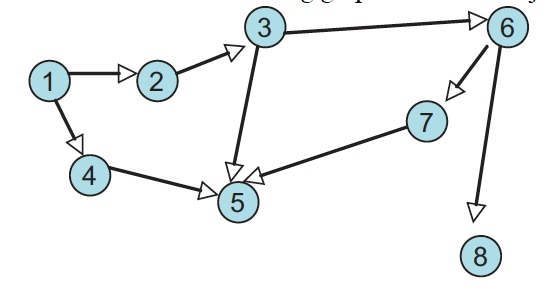
\includegraphics[width=0.95\textwidth]{graph}
  \caption{Graph -- question 4}
\end{figure}

\begin{table}[H]
  \centering
  \subfloat[Adjacency matrix\label{table:four:adjacency}]{
    \begin{tabular}{ | c | c | c | c | c | c | c | c | c | }
      \hline
      \neun{}{1}{2}{3}{4}{5}{6}{7}{8}
      1 & 1 & 1 & 0 & 1 & 0 & 0 & 0 & 0 \\
      2 & 0 & 1 & 1 & 0 & 0 & 0 & 0 & 0 \\
      3 & 0 & 0 & 1 & 0 & 1 & 1 & 0 & 0 \\
      4 & 0 & 0 & 0 & 1 & 1 & 0 & 0 & 0 \\
      5 & 0 & 0 & 0 & 0 & 1 & 0 & 0 & 0 \\
      6 & 0 & 0 & 0 & 0 & 0 & 1 & 1 & 1 \\
      7 & 0 & 0 & 0 & 0 & 1 & 0 & 1 & 0 \\
      8 & 0 & 0 & 0 & 0 & 0 & 0 & 0 & 1 \\
      \hline
    \end{tabular}
  }

  \subfloat[Edge list\label{table:four:edgeList}]{
    \begin{tabular}{ | c | c | }
      \hline
      \zwei{Node}{Edges}
      \edgeinfo{1:}{2,4}
      \edgeinfo{2:}{3}
      \edgeinfo{3:}{5,6}
      \edgeinfo{4:}{5}
      \edgeinfo{5:}{\emptyset}
      \edgeinfo{6:}{7,8}
      \edgeinfo{7:}{5}
      \edgeinfo{8:}{\emptyset}
      \hline
    \end{tabular}
  }
  \caption[graphs]{Adjacency matrix \& edge list -- question 4}
\end{table}

%------------------------------------------------------

\section[question_5]{Construct a graph in which a depth first search will
  uncover a solution (discover reachability from one vertex to another) in
  fewer steps than will a breadth first search. You may need to specify an
  order in which neighbor vertices are visited. Construct another graph in
  which a breadth-first search will uncover a solution in fewer steps.}




%------------------------------------------------------

\section[question_6]{Complete Worksheet 41 (2 simulations). Show the content
  of the stack, queue, and the set of reachable nodes.}

\setcounter{subtable}{0}
\begin{table}[H]
  \centering
  \subfloat[Worksheet 41 -- DFS (Stack)\label{table:worksheet41_DFS}]{
    \begin{tabular}{ | c | l | l | }
      \hline
      \drei{Iteration}{Stack (T -- B)}{Reachable}
      \wsinfo{0}{1}{}
      \wsinfo{1}{6,2}{1}
      \wsinfo{2}{11,2}{1,6}
      \wsinfo{3}{16,12,2}{1,6,11}
      \wsinfo{4}{21,12,2}{1,6,11,16}
      \wsinfo{5}{22,12,2}{1,6,11,16,21}
      \wsinfo{6}{23,17,12,2}{1,6,11,16,21,22}
      \wsinfo{7}{17,12,2}{1,6,11,16,21,22,23}
      \wsinfo{8}{12,12,2}{1,6,11,16,21,22,23,17}
      \wsinfo{9}{13,12,2}{1,6,11,16,21,22,23,17,12}
      \wsinfo{10}{18,8,12,2}{1,6,11,16,21,22,23,17,12,13}
      \wsinfo{11}{8,12,2}{1,6,11,16,21,22,23,17,12,13,18}
      \hline
    \end{tabular}
  }

  \subfloat[Worksheet 41 -- BFS (Queue)\label{table:worksheet41_BFS}]{
    \begin{tabular}{ | c | l | l | }
      \hline
      \drei{Iteration}{Queue (F -- B)}{Reachable}
      \wsinfo{0}{1}{}
      \wsinfo{1}{2,6}{1}
      \wsinfo{2}{6,3,7}{1,2}
      \wsinfo{3}{3,7,11}{1,2,6}
      \wsinfo{4}{7,11,4,8}{1,2,6,3}
      \wsinfo{5}{11,4,8}{1,2,6,3,7}
      \wsinfo{6}{4,8,12,16}{1,2,6,3,7,11}
      \wsinfo{7}{8,12,16,5,9}{1,2,6,3,7,11,4}
      \wsinfo{8}{12,16,5,9,13}{1,2,6,3,7,11,4,8}
      \wsinfo{9}{16,5,9,13,13,17}{1,2,6,3,7,11,4,8,12}
      \wsinfo{10}{5,9,13,13,17,21}{1,2,6,3,7,11,4,8,12,16}
      \wsinfo{11}{9,13,13,17,21,10,14}{1,2,6,3,7,11,4,8,12,16,5}
      \wsinfo{12}{13,13,17,21,10,14}{1,2,6,3,7,11,4,8,12,16,5,9}
      \wsinfo{13}{13,17,21,10,14,18}{1,2,6,3,7,11,4,8,12,16,5,9,13}
      \hline
    \end{tabular}
}
\caption[worksheet41]{Worksheet 41 -- question 6}
\end{table}

%------------------------------------------------------

\section[question_7]{Complete Worksheet 42 (1 simulation). Show the content of
  the priority queue and the cities visited at each step.}

\begin{table}[H]
  \centering
  \begin{tabular}{ | c | l | l | }
    \hline
    \drei{Iteration}{Priority queue}{Added to reachable}
    \wsinfo{0}{Pensacola(0)}{}
    \wsinfo{1}{Phoenix(5)}{Pensacola(0)}
    \wsinfo{2}{Pueblo(8), \ Peoria(9), \ Pittsburgh(15)}{Phoenix(5)}
    \wsinfo{3}{Peoria(9), \ Pierre(11), \ Pittsburgh(15)}{Pueblo(8)}
    \wsinfo{4}{\makecell[l]{Pierre(11), \ Pueblo(12), \ Pittsburgh(14), \\
    Pittsburgh(15)}}{Peoria(9)}
    \wsinfo{5}{\makecell[l]{Pueblo(12), \ Pendleton(13), \ Pittsburgh(14), \\
    Pittsburgh(15)}}{Pierre(11)}
    \wsinfo{6}{Pendleton(13), \ Pittsburgh(14), \ Pittsburgh(15)}{}
    \wsinfo{7}{\makecell[l]{Pittsburgh(14), \ Pittsburgh(15), \ Phoenix(19), \\
    Pueblo(21)}}{Pendleton(13)}
    \wsinfo{8}{\makecell[l]{Pittsburgh(15), \ Pensacola(18), \ Phoenix(19), \\
    Pueblo(21)}}{Pittsburgh(14)}
    \wsinfo{9}{\makecell[l]{Pensacola(18), \ Phoenix(19), \ Pensacola(19), \\
    Pueblo(21)}}{}
    \wsinfo{10}{Phoenix(19), \ Pensacola(19), \ Pueblo(21)}{}
    \wsinfo{11}{Pensacola(19), \ Pueblo(21)}{}
    \wsinfo{12}{Pueblo(21)}{}
    \wsinfo{13}{}{}
    \hline
  \end{tabular}
  \caption[worksheet42]{Worksheet 42 -- question 7}
\end{table}

%------------------------------------------------------

\section[question_8]{Why is it important that Dijkstra's algorithm stores
  intermediate results in a priority queue, rather than in an ordinary stack
  or queue?}

It is important, because the intent is to take the path with the lowest
associated cost -- prioritizing intermediate edges -- which is a property that
neither a stack nor a queue posses. of the three, only a priority queue
possesses this property (this is also assuming that priorities are
determined by cumulative cost from the point of origin).

%------------------------------------------------------

\section[question_9]{How much space (in big-O notation) does an edge-list
  representation of a graph require?}

$O (\abs{V} + \abs{E})$

%------------------------------------------------------

\section[question_10]{For a graph with V vertices, how much space (in big-O
  notation) will an adjacency matrix require?}

$O \abs{V}^2$

%------------------------------------------------------

\section[question_11]{Suppose you have a graph representing a maze that is
  infinite in size, but there is a finite path from the start to the
  finish. Is a depth first search guaranteed to find the path? Is a
  breadth-first search guaranteed to find the path? Explain why or why not.}

For an infinite size maze, a \emph{depth-first search} does not guarantee this
path will be found. This algorithm will search along a path until it reaches
an end, and since the size of the maze can be infinite, it is possible for the
path of a depth-first search to be infinitely long. \\

However, using a \emph{breadth-first search} does guarantee the path will be
found, because this algorithm will search the nearest neighbor points --
beginning with the starting point -- and gradually enlarge the search
region. This ensures that the finite path you are looking for will eventually
be found.

%------------------------------------------------------

\end{document}

%%% Local Variables:
%%% mode: latex
%%% TeX-master: t
%%% End:
